%----------------------------------------------------------------------------------------
%	Inställningar och dokumentkonfiguration
%----------------------------------------------------------------------------------------

\documentclass[paper=a4, fontsize=11pt]{report} % A4-sida och 11 punkters fontstorlek

\usepackage[T1]{fontenc} % 8-bitarskodning som har 256 glyfer
\usepackage[english]{babel} % Svenskt språk(ändrat till engelska)
\usepackage[utf8]{inputenc} % För svenska tecken
\usepackage{dtklogos} % Logos
\usepackage{wallpaper} % Bakgrundsbild
\usepackage{fancyhdr} % Specialsidhuvud och sidfot
\usepackage{enumerate} 
\usepackage{hyperref}
\usepackage{textcomp}
\usepackage{xifthen}% provides \isempty test
\pagestyle{fancyplain} % Använd sidhuvud och sidfot på alla sidor
\fancyhead[L]{Laboration 3 -- 1DV020 -- VT15 -- Server administraion I} % Titel till vänster i sidhuvud
\fancyhead[C]{} % Tomt i mitten
\fancyhead[R]{} % Tomt till höger
\fancyfoot[L]{{\color{gray}\textcopyright \ 2015 Jacob Lindehoff, Kristoffer Schill}} % Tomt till vänster
\fancyfoot[C]{}  % Tomt i mitten
\fancyfoot[R]{\thepage} % Sidnumrering till höger i sidfoten
\renewcommand\thesection{\arabic{section}} % Section beter sig som i dokumentklassen article

\newcommand{\win}[1]{Microsoft Windows Server\ifthenelse{\isempty{#1}}{}{ #1}}
\newcommand{\gui}[0]{``Server with a GUI''}
\newcommand{\core}[0]{Windows Server Core}
%----------------------------------------------------------------------------------------
%	TITLE SECTION
%----------------------------------------------------------------------------------------
\newcommand\BackgroundPic{
    \put(-50,-50){
    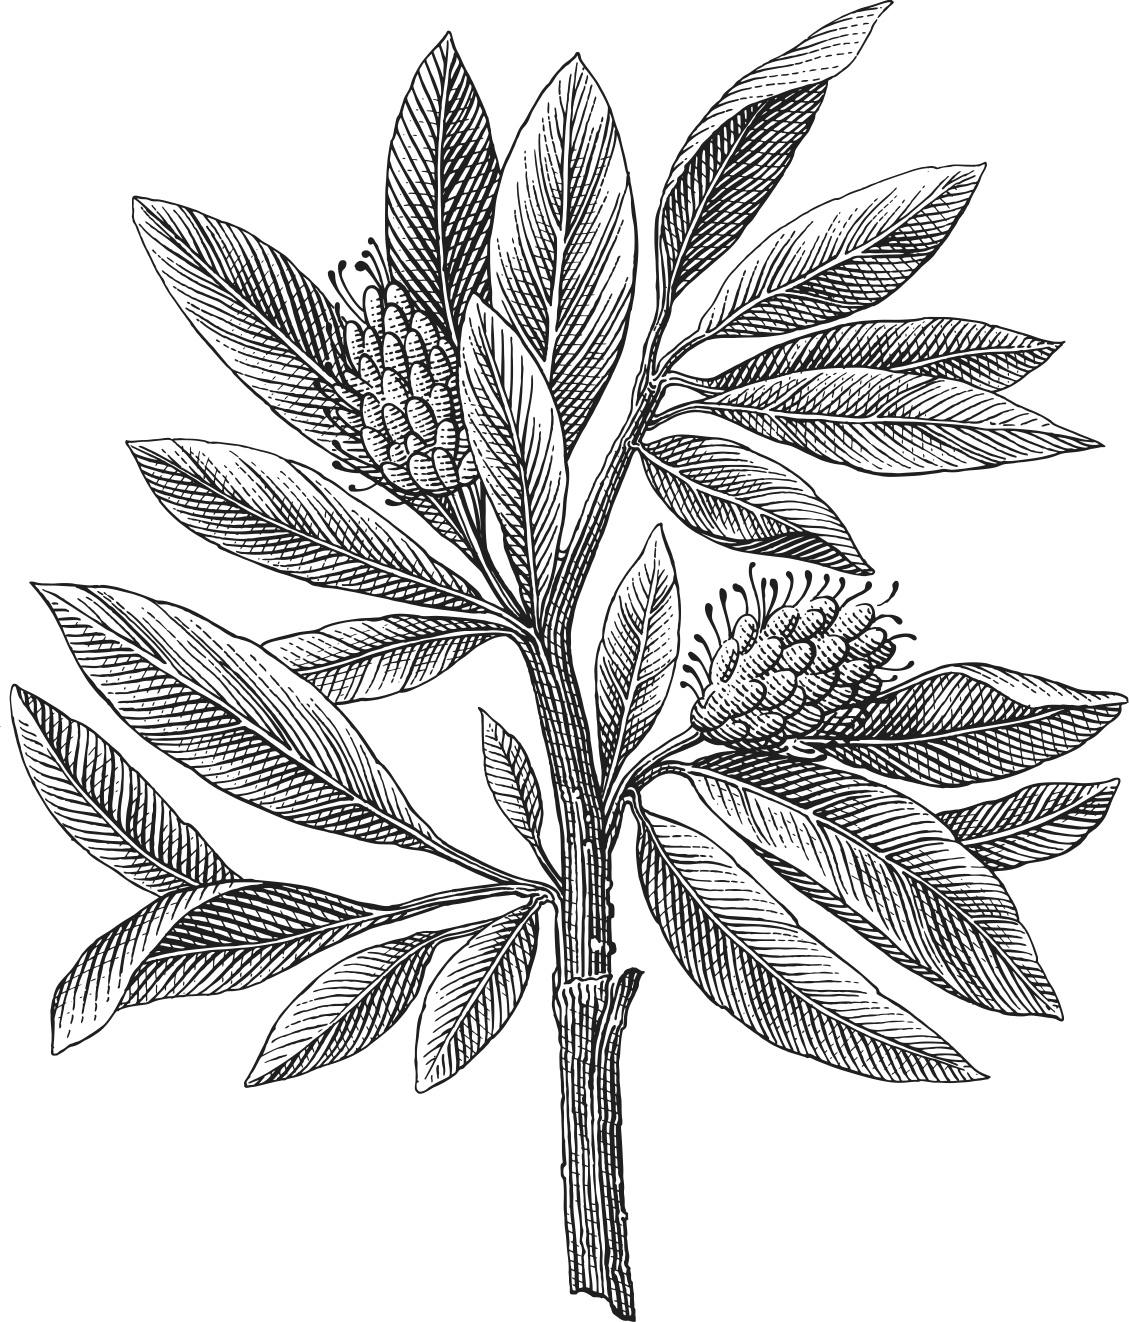
\includegraphics[keepaspectratio,scale=0.65]{lnu_etch.png} % Bakgrundsbild
    }
}
\newcommand\BackgroundPicLogo{
    \put(15,700){
    
\includegraphics[keepaspectratio,scale=0.10]{logo.png} % Logga i vänstra hörnet
    }
}

\newcommand{\horrule}[1]{\rule{\linewidth}{#1}} % Skapa hortisontell linje

\title{	\vspace{-10cm}
    \normalfont \normalsize
    \textsc{Linnéuniversitetet} \\ [25pt] % Universitetes namn
    \horrule{0.5pt} \\[0.4cm] % Tunn linje högst upp
    \huge Laboration 3\\ % Arbetes titel
	\large \textcolor{gray}{1DV020 -- Serveradministraion}
    \horrule{0.5pt} \\[0.4cm] % Tunn linje längst ner
}

% \author{Jacob Lindehoff} % Författarnas namn

\date{\normalsize\today} % Dagens datum

\begin{document}
\AddToShipoutPicture*{\BackgroundPic} % Lägger in backgrundsbild på första sidan
\AddToShipoutPicture*{\BackgroundPicLogo}
\maketitle % Skriv ut titeln
\noindent % Tabba inte in på första meningen

%------------------------------------------------
%	Introduction
%------------------------------------------------
\section{Introduction}

In this Laboration we will cover 3 concepts: DHCP, DNS and a Web server - and see how they work together. As previously we will be using the lab from where we left off. We will also introduce a new VMNet (5) and add another server there - dmzserver.

Our previous Linux server will act as a DNS for mycompany.lab. The new dmzserver will act as our web server for mycompany.lab and the windows server will be responsible for handing out IP addresses with DHCP.

%------------------------------------------------
%	Deadline
%------------------------------------------------
\section{Deadline}

There are two laboratory sessions connected to this module, at these sessions you are given the opportunity to get help if so needed. To be able to finish the modules you are likely needed to spend more time on your own.

\paragraph{Accounting} You will show your work and demonstrate your progress at any of these lab session, prepare a small document with an overview of your configuration/setup if needed for overview.

\pagebreak
%------------------------------------------------
%	Uppgift
%------------------------------------------------
\section{Assignment}
The following fours sections with subtasks are the assignment:

\subsection{Add a second virtual machine and VMNet}
We will add another VMNet (5) that will act as our DMZ and put a virtual Linux server on it from here on called \textbf{dmzserver}.  To do this and make it communicate with our network we need to manually add another network interface on our linux router on VMNet 5, see figure \figurename \ref{fig:network}.
\begin{figure}[h]
\centering
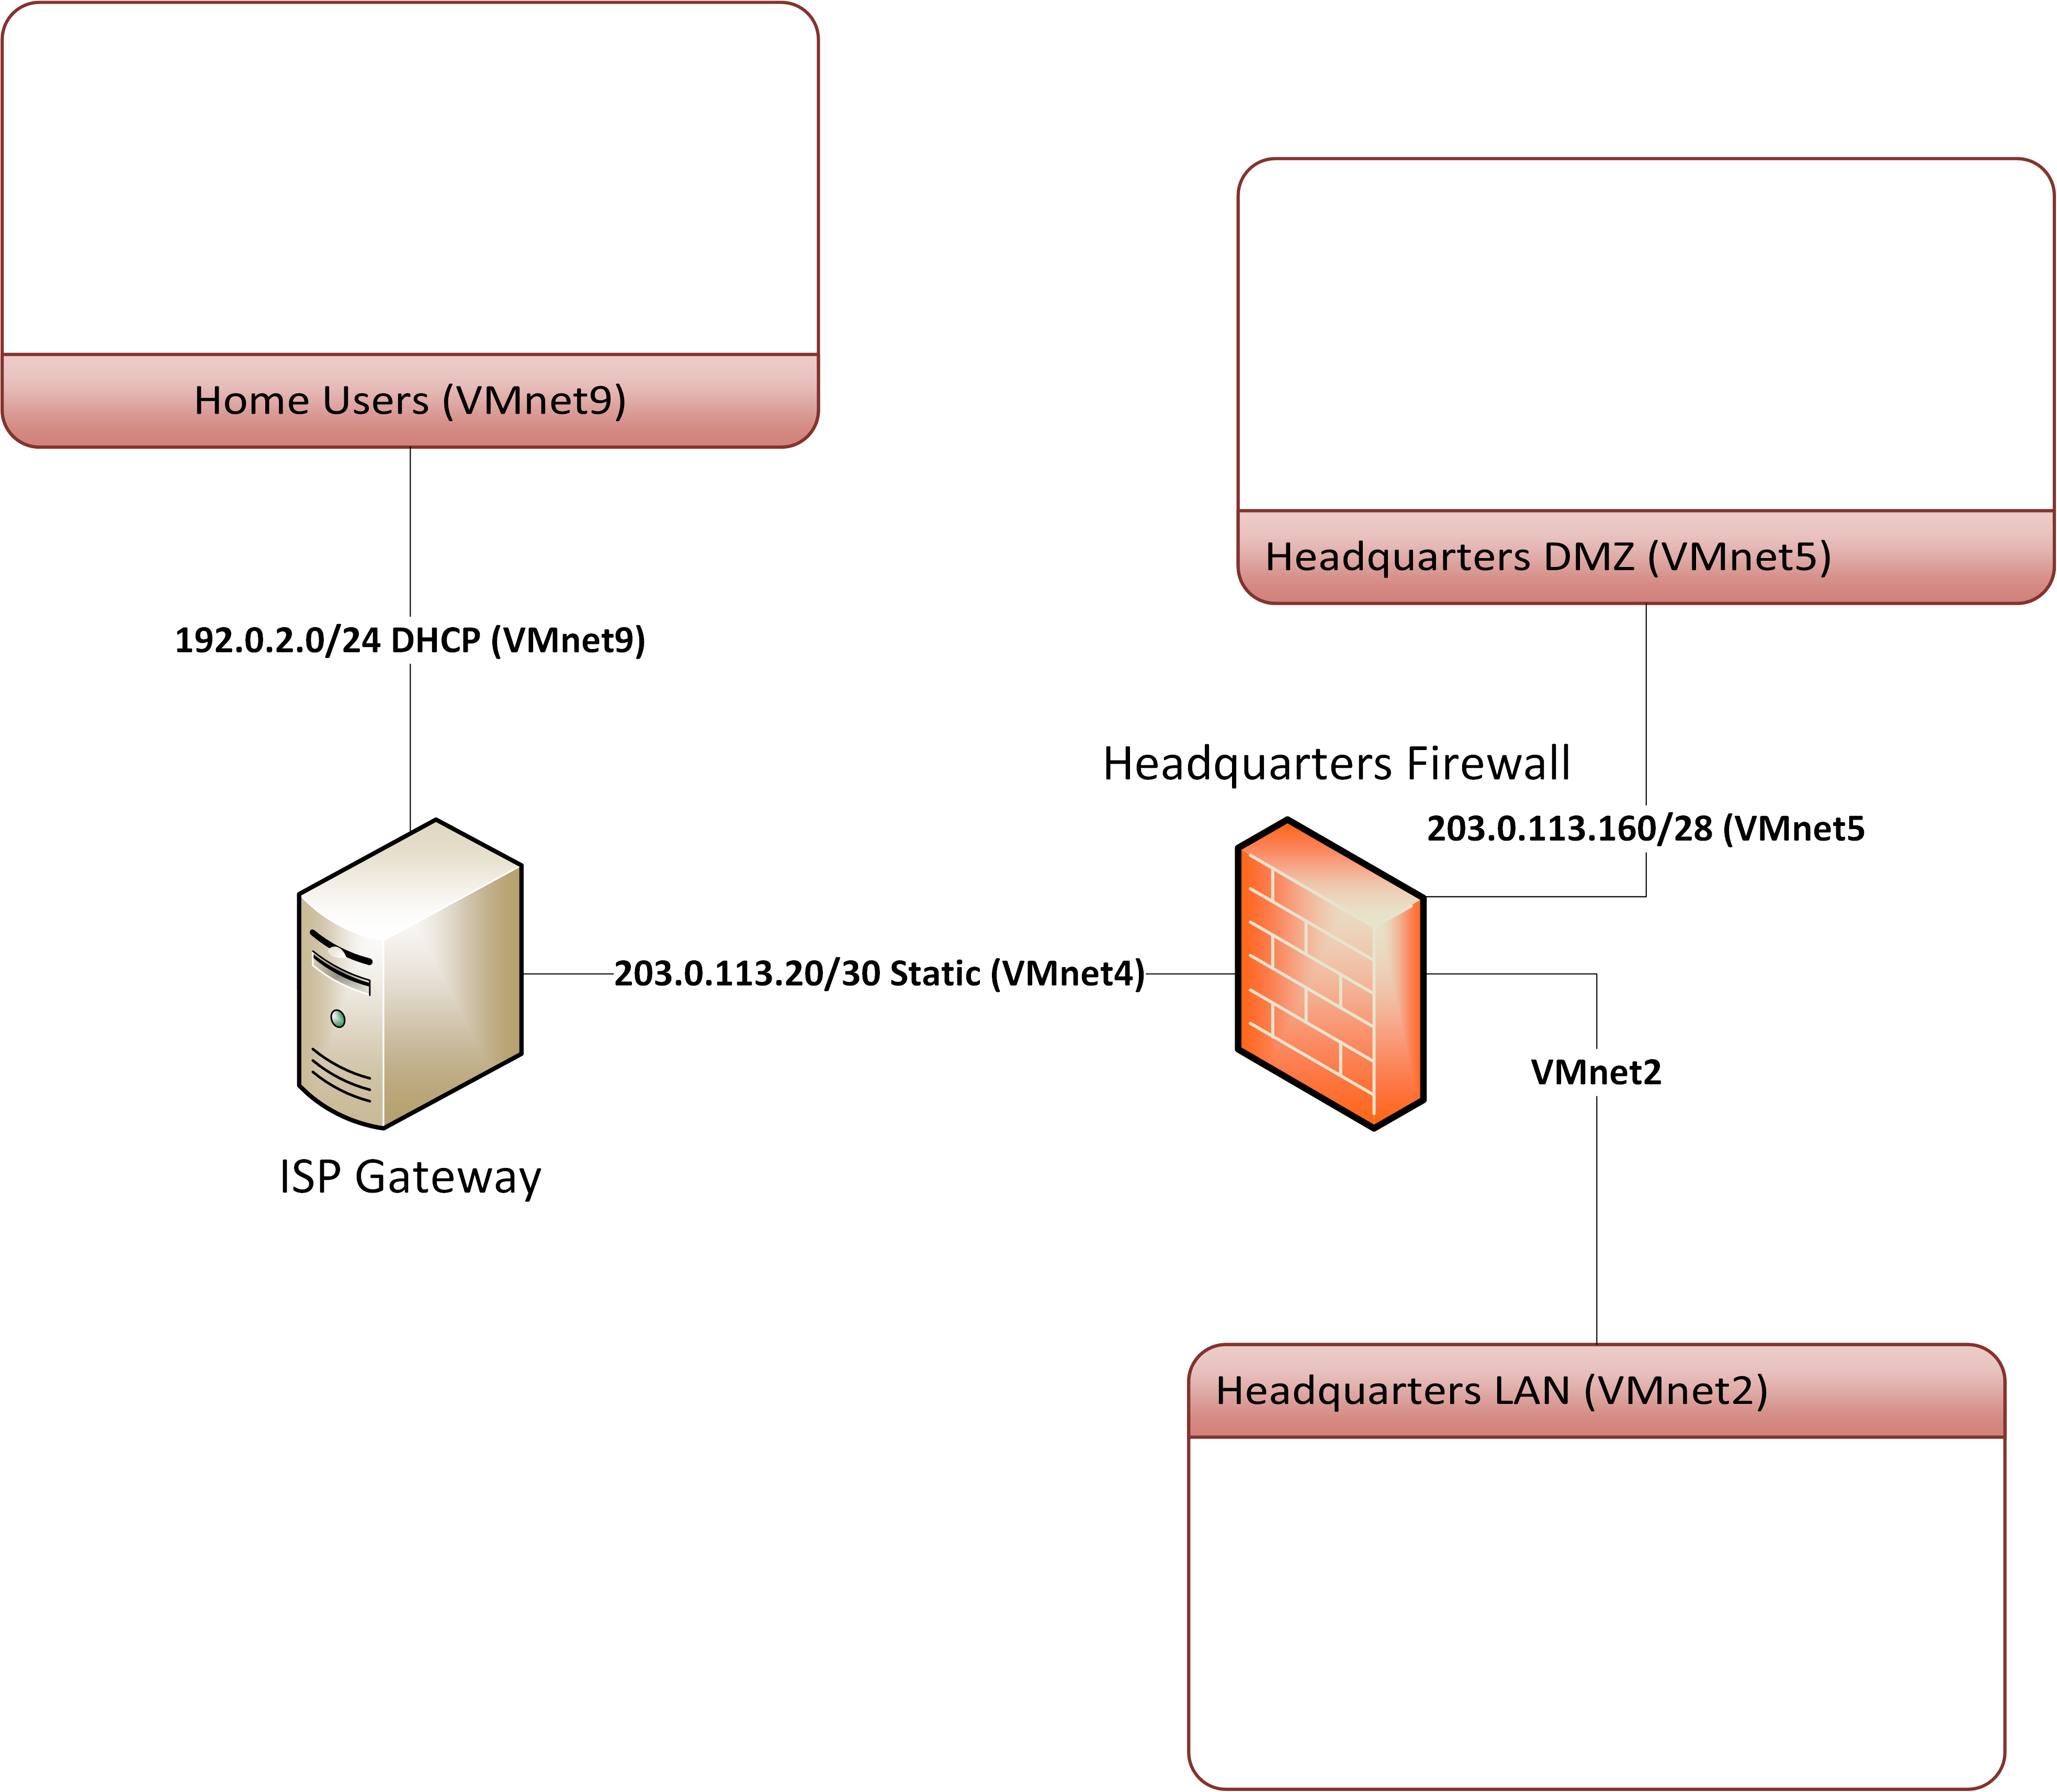
\includegraphics[width=1\linewidth]{./network}
\caption[Figure over network in Lab 3]{The network as it should be setup in Lab 3.}
\label{fig:network}
\end{figure}
We also need to put this VMNet 5 in the subnet 203.0.113.160/28 this is because the ISP gateway is configured to route this traffic to VMNet 4 toward the firewall You should be able to ping the machine from both VMNet 9 ,4 and 2.
\subsection{DNS}
First install bind9, bind9utils and dnsutils
\begin{enumerate}
	\item Turn your internal linux server into a forward and caching DNS-server.  Don’t forget to point the forwarder to 203.0.113.21. You should also point the machines DNS to the localhost 127.0.0.1 (in the same matter as you pointed it to 203.0.113.21 in the first module.)
		To confirm it is actually caching the data you can use: rndc dumpdb. And locate the cache in: /var/cache/bind/named\_dump.db
	\item We now setup and make records for our internal network: corp.mycompany.lab. It  should contain records for:
		\begin{itemize}
			\item the linux server
			\item the windows server
			\item the internal gateway.
			\item reverse lookup for those hosts.
		\end{itemize}
		\item Make the linux server authoritative over mycompany.lab It should at least contain the following records using A or A + CNAME records:
			\begin{itemize}
				\item www -> <dmz server>
				\item altwww -> <dmz server>
				\item company -> 203.0.113.22
			\end{itemize}
		\item Now that we see that we have our own zone we will register it to the ISP. To do this use a computer that refers to the ISP gateway as its DNS server 203.0.113.21 (should be all computers within your virtual environment) and direct one of their browsers to www.nic.lab . here you will be able to register a domain.
			
			For the registration to work the DNS server needs to be correctly configured. When asked asked for a name server you direct it to: hq-ip-gw.static.lab (This is just an A record pointing to your linux routers external ip 203.0.113.22.)
			
			Don’t forget that the DNS traffic (port 53) going from the ISP gateway needs to be forwarded to your internal linux server
\end{enumerate}

\subsection{DHCP}
For the DHCP part we will be using the windows server as our DHCP server handing out ip addresses. the first thing is to install the role. Then we will be using the MAC address for our internal computers (except the router) and reserve the IP for the Ubuntu server using the MAC address of the interfaces. You can find the MAC address either on the virtual network adapter ( Virtual Machine Settings -> Network Adapter -> Advanded) or on the machine itself.

The ubuntu server and the internal client should not need to specify gateway or DNS manually. All this should be handled by the DHCP server.

\subsection{Web server}
Install a web server on your newly created \textbf{dmzserver} on VMNet 5.
\begin{enumerate}
	\item Then setup two virtual hosts on that server. If your DNS settings are correct you should be able to reach the web server from any browser on the network using the following addresses:
		\begin{itemize}
			\item www.mycompany.lab
			\item altwww.mycompany.lab
		\end{itemize}
		so www.mycompany.lab should show one page and then altwww.mycompany.lab another.
	\item Make a third page that is only seen when you connect to it using the port 2015.
		All pages should of course be reachable at the same time.
\end{enumerate}


\section{Requirements}
Consider not using the firewall at all when implementing but instead add the rules once you see that all is working. Otherwise it should work as in the assignment description. 

\section{Workenviroment}
\label{enviroment}
We will continue to use the lab where we left of. If you get stuck somewhere you can try your luck with another part but to configure DHCP properly you at least need to be done with forwarding part of the DNS (so we can refer to the linux server as our DNS). And to get the virtual hosts working we need the DNS records(unless we circumvent it mapping local hosts)

Good luck!
\end{document}
